%standard 5.2


%start_of_questions

%new_question
%%%%%%%%%%%%%%%%%%%%%
	% Problem 1
	% Difficulty: 2
%%%%%%%%%%%%%%%%%%%%%
	\item
		Write a \textbf{function} that calculates then returns the volume of a right square pyramid.  
		The arguments of the function will be $b$ (the base edge) and $h$ (the height).\\
		Use the value of $\pi$ from the math module in your calculation.\\	
		Hint: $V = \dfrac{b^2 h}{3}$

\begin{tabular}{l c}
	\begin{minipage}{0.5\textwidth}
	\textbf{Examples:}
		\begin{itemize}
			\item  pyramid\_volume(1, 2) $\rightarrow$ 0.66, 
			\item  pyramid\_volume(2, 2) $\rightarrow$ 2.66, 
			\item  pyramid\_volume(3, 4) $\rightarrow$ 12 
		\end{itemize}
	\end{minipage}

	\begin{minipage}{0.4\textwidth}
		\begin{flushright}
		\tdplotsetmaincoords{70}{-20}
		\begin{tikzpicture}[tdplot_main_coords,line cap=butt,line join=bevel]
			\pgfmathsetmacro{\B}{4}
			\pgfmathsetmacro{\H}{4}
			\draw[thick] (-\B/2,-\B/2,0) -- (\B/2,-\B/2,0) -- (\B/2,\B/2,0) -- (-\B/2,\B/2,0)
				 -- cycle;
			\draw[thick] (\B/2,\B/2,0) -- (0,0,\H)
			node[above,font=\large\bfseries]{};
			\draw[dashed] (0,0,0) -- (0,0,\H) coordinate[midway](aux1);
			\draw[] (0,0,0.3) -- (0.3,0,0.3) -- (0.3,0,0);
			%\draw[dashed,blue] (-\B/2,0,0) -- (0,0,\H) coordinate[pos=0.3](aux2);
			%\draw[blue] ({-\B/2+0.15*(\H/\B)},0,0.3) -- ({-\B/2+0.15*(\H/\B)},-0.3,0.3) 
				%-- (-\B/2,-0.3,0);
			\coordinate (aux3) at (0.3,-2,0);
			\draw[thick] (-\B/2,-\B/2,0) -- (0,0,\H) -- (\B/2,-\B/2,0) -- cycle;
			\draw[thick] (-\B/2,-\B/2,0) -- (0,0,\H) -- (-\B/2,\B/2,0) -- cycle;
			\begin{scope}[tdplot_screen_coords]
				\draw (aux1) -- ++ (2,0.1) node[right,font=\itshape] {Height: h};
				%\draw (aux2) -- ++ (-1.5,0.3) node[left,font=\itshape] {Slant Height};
				\draw (aux3) -- ++ (2,-0.2) node[below right,font=\itshape] {Base edge: b};
			\end{scope}
		\end{tikzpicture}
		\end{flushright}
\end{minipage}
\end{tabular}


%new_question
%%%%%%%%%%%%%%%%%%%%%
	% Problem 2
	% Difficulty: 2
%%%%%%%%%%%%%%%%%%%%%
	\item
		Write a \textbf{function} that calculates then returns the volume of a cone.  \\
		The arguments of the function will be $r$ (the radius) and $h$ (the height).\\
		Use the value of $\pi$ from the math module in your calculation.\\	
		Hint: $V = \pi \cdot \dfrac{r^2 h}{3}$

\begin{tabular}{l c}
	\begin{minipage}{0.5\textwidth}
	\textbf{Examples:}
		\begin{itemize}
			\item  cone\_volume(1, 2) $\rightarrow$ 2.09, 
			\item  cone\_volume(3, 3) $\rightarrow$ 28.27, 
			\item  cone\_volume(1, 4) $\rightarrow$ 4.18 
		\end{itemize}
	\end{minipage}

	\begin{minipage}{0.4\textwidth}
		\begin{flushright}
		\begin{tikzpicture}
			\draw[dashed] (0,0) arc (170:10:2cm and 0.4cm)coordinate[pos=0] (a);
			\draw (0,0) arc (-170:-10:2cm and 0.4cm)coordinate (b);
			\draw[densely dashed] ([yshift=4cm]$(a)!0.5!(b)$) 
				-- node[right,font=\footnotesize]{$h$}coordinate[pos=0.95] (aa)($(a)!0.5!(b)$)
				-- node[below,font=\footnotesize] {$r$}coordinate[pos=0.1] (bb) (b);
    		\draw (aa) -| (bb);
    		\draw (a) -- ([yshift=4cm]$(a)!0.5!(b)$) -- (b);
  		\end{tikzpicture}
	\end{flushright}
\end{minipage}
\end{tabular}

%new_question
%%%%%%%%%%%%%%%%%%%%%
	% Problem 3
	% Difficulty: 2
%%%%%%%%%%%%%%%%%%%%%
	\item 
		You are counting points for a basketball game. Write a \textbf{function} that 
		calculates the final points for the team and returns the value. The arguments for the function will be 
		$two\_pointers$ (number of two-pointers scored) and $three\_pointers$ (number of three-pointers scored).\\

	\textbf{Examples:}
	\begin{itemize}
		\item total\_score(5, 7) $\rightarrow$ 31, 
		\item total\_score(6, 5) $\rightarrow$ 27, 
		\item total\_score(10, 10) $\rightarrow$ 50 
	\end{itemize}

%new_question
%%%%%%%%%%%%%%%%%%%%%
	% Problem 4
	% Difficulty: 2
%%%%%%%%%%%%%%%%%%%%%
	\item 
		You are counting points for a tennis match. Write a \textbf{function} that 
		calculates the total points for a player and returns the value. The arguments for the function will be 
		$aces$ (each ace is worth 2 points) and $winning\_shots$ (each winning shot is worth 1 point).\\

	\textbf{Examples:}
	\begin{itemize}
		\item total\_score(1, 1) $\rightarrow$ 3, 
		\item total\_score(2, 3) $\rightarrow$ 7, 
		\item total\_score(5, 3) $\rightarrow$ 13
	\end{itemize}

%new_question
%%%%%%%%%%%%%%%%%%%%%
	% Problem 5
	% Difficulty: 2
%%%%%%%%%%%%%%%%%%%%%
	\item 
		A farmer is asking you to tell him how many legs can be counted among all his animals. 
		The farmer breeds three species:
		\begin{itemize}
			\item chickens, which have \textbf{2} legs
			\item cows, which have \textbf{4} legs
			\item pigs, which have \textbf{4} legs
		\end{itemize}
		Write a \textbf{function} that counts the total number of legs in the farmer's land and returns the value. 
		The arguments for the function will be chickens (number of chickens farmer has), cows (number of cows farmer has), and pigs (number of pigs farmer has).\\

	\textbf{Examples:}
	\begin{itemize}
		\item  leg\_counter(4, 3, 2) $\rightarrow$ 28, 
		\item  leg\_counter(1, 1, 1) $\rightarrow$ 10, 
		\item  leg\_counter(0, 10, 0) $\rightarrow$ 40 
	\end{itemize}

%new_question
%%%%%%%%%%%%%%%%%%%%%
	% Problem 6
	% Difficulty: 2
%%%%%%%%%%%%%%%%%%%%%
	\item 
		A toy store owner wants to know the total number of batteries needed for all the electronic toys in the store. 
		The store sells three types of toys:
		\begin{itemize}
			\item Electronic dolls, which require \textbf{2} batteries
			\item Remote-controlled cars, which require \textbf{4} batteries
			\item Robot dogs, which require \textbf{6} batteries
		\end{itemize}


		Write a \textbf{function} that counts the total number of batteries needed for the toy store and returns the value. 
		The arguments for the function will be $e\_dolls$ (number of electronic dolls toy store has), $rc\_cars$ 
		(number of remote-controlled cars toy store has), and $robo\_dogs$ (number of robot dogs toy store has).\\

	\textbf{Examples:}
	\begin{itemize}
		\item  battery\_counter(4, 3, 2) $\rightarrow$ 32, 
		\item  battery\_counter(1, 1, 1) $\rightarrow$ 12, 
		\item  battery\_counter(0, 10, 0) $\rightarrow$ 40 
	\end{itemize}


%new_question
%%%%%%%%%%%%%%%%%%%%%
	% Problem 7
	% Difficulty: 2
%%%%%%%%%%%%%%%%%%%%%
	\item 
		The table below show what your resting heart rate should be based on age and athleticism. 
		Write a \textbf{function} that returns what the resting heart rate of the user should be. 
		The arguments for the function will be $age$ (how old the user is) and $athl\_goal$ (athletic goal of user).
	\begin{center}
		\begin{minipage}{.45\textwidth}
			\begin{tabular}{c|cc}
				& \multicolumn{2}{c}{Athleticism}\\
				Age & Above Average & Below Average \\ \hline
				20 -- 39 & 47 -- 72 & 73 -- 93\\
				40 -- 59 & 46 -- 71 & 72 -- 94\\
				60 -- 79 & 45 -- 70 & 71 -- 97 \\
			\end{tabular}
		\end{minipage}
	\end{center}

	\textbf{Examples:}
	\begin{itemize}
		\item  resting\_rate(45, \csq{Below Average}) $\rightarrow$ \csq{72-94}, 
		\item  resting\_rate(79, \csq{Above Average}) $\rightarrow$ \csq{45-70}, 
		\item  resting\_rate(20, \csq{Below Average}) $\rightarrow$ \csq{73-93} 
	\end{itemize}


%new_question
%%%%%%%%%%%%%%%%%%%%%
	% Problem 8
	% Difficulty: 2
%%%%%%%%%%%%%%%%%%%%%
	\item 
		The table below shows what time different age groups (by grade) can swim at the pool.  There 
		are two time options, morning and afternoon.  Write a \textbf{function} that returns the time 
		the pool is available for the user. The arguments for the function will be $grade$ (which grade the user is in) 
		and $time$ (which time the user would like to go in).
	\begin{center}
		\begin{minipage}{.45\textwidth}
			\begin{tabular}{c|cc}
				& \multicolumn{2}{c}{Pool times}\\
				Grade 		& Morning 	& Afternoon \\ \hline
				k, 1 -- 3 	& 9 AM 		& 1 PM\\
				4 -- 8 		& 10 AM 	& 2 PM\\
				9 -- 12 	& 11 AM 	& 3 PM \\
			\end{tabular}
		\end{minipage}
	\end{center}

	\textbf{Examples:}
	\begin{itemize}
		\item  pool\_time('k', \csq{Morning}) $\rightarrow$ \csq{9 AM}, 
		\item  pool\_time(5, \csq{Afternoon}) $\rightarrow$ \csq{2 PM}, 
		\item  pool\_time(12, \csq{Morning}) $\rightarrow$ \csq{11 AM}
	\end{itemize}


%new_question
%%%%%%%%%%%%%%%%%%%%%
	% Problem 15
	% Difficulty: 2
%%%%%%%%%%%%%%%%%%%%%
	\item 
		%https://edabit.com/challenge/b8wRDMWgMZTN2nmfx
		Write a \textbf{function} that returns the number of copies of the same number. The arguments for the function will be $num\_1$ (first number), 					$num\_2$ (second number), and $num\_3$ (third number).\\

		\textbf{Examples:}		
		\begin{itemize}
			\item  count\_duplicates(2, 3, 2) $\rightarrow$ \csq{You entered the same number 2 times}, 
			\item  count\_duplicates(4, 4, 4) $\rightarrow$ \csq{You entered the same number 3 times}, 
			\item  count\_duplicates(1, 2, 3) $\rightarrow$ \csq{Each number is unique} 
		\end{itemize}



%new_question
%%%%%%%%%%%%%%%%%%%%%
	% Problem 20
	% Difficulty: 2
%%%%%%%%%%%%%%%%%%%%%
	\item 
		%https://edabit.com/challenge/sfqudQHQ3HPpd7dZb
		Write a \textbf{function} to create a game of Rock, Paper, Scissors. The function will return the winner of the game played by two players.
		The arguments to the function will be $player1$ (the first player's choice) and $player2$ (the second player's choice).\\
		Print the winner according to the following rules. 
		\begin{itemize}
			\item Rock beats Scissors
			\item Scissors beats Paper
			\item Paper beats Rock
		\end{itemize}		
		\textbf{Examples:}		
		\begin{itemize}
			\item  find\_winner(\csq{Rock}, \csq{Paper}) $\rightarrow$ \csq{Player 2 wins!}, 
			\item  find\_winner(\csq{Scissors}, \csq{Paper}) $\rightarrow$ \csq{Player 1 wins!}, 
			\item  find\_winner(\csq{Rock}, \csq{Rock}) $\rightarrow$ \csq{It's a tie!}
		\end{itemize}


%new_question
%%%%%%%%%%%%%%%%%%%%%
	% Problem 21
	% Difficulty: 2
%%%%%%%%%%%%%%%%%%%%%
	\item 
		%https://edabit.com/challenge/ancAxGEF9MsLWXDqe
		Write a \textbf{function} that returns if a triangle is a scalene, isosceles, or an equilateral. The arguments to the function will be 
		$side\_1$ (first side of the triangle), $side\_2$ (second side of the triangle), and $side\_3$ (third side of the triangle).\\
		The types of triangles are: 
		\begin{itemize}
			\item No sides equal: \csq{scalene}
			\item Two sides equal: \csq{isosceles}
			\item All sides equal: \csq{equilateral}	
		\end{itemize}
		\textbf{Examples:}		
		\begin{itemize}
			\item  triangle\_type(1, 2, 3) $\rightarrow$ \csq{scalene}, 
			\item  triangle\_type(4, 4, 4) $\rightarrow$ \csq{equilateral}, 
			\item  triangle\_type(7, 7, 3) $\rightarrow$ \csq{isosceles} 
		\end{itemize}


%new_question
%%%%%%%%%%%%%%%%%%%%%
	% Problem 26
	% Difficulty: 2
%%%%%%%%%%%%%%%%%%%%%
	\item 
		Write a \textbf{function} that loops through and prints every even number between two
		integers (inclusive). The arguments to the function will be $smaller\_num$ and 
		$larger\_num$.

		\textbf{Examples:}		
		\begin{itemize}
			\item  output\_even(37, 1050) $\rightarrow$ 38, 40, 42, \dots 1048, 1050, 
			\item  output\_even(1, 2000) $\rightarrow$ 2, 4, 6, \dots 1998, 2000 
			\item  output\_even(50, 199) $\rightarrow$ 50, 52, 54, \dots 196, 198
		\end{itemize}


%new_question
%%%%%%%%%%%%%%%%%%%%%
	% Problem 27
	% Difficulty: 2
%%%%%%%%%%%%%%%%%%%%%
	\item 
		Write a \textbf{function} that loops through and returns the sum of all odd numbers 
		between two integers (inclusive). The arguments to the function will be $smaller\_num$ 
		and $larger\_num$.

		\textbf{Examples:}		
		\begin{itemize}
			\item  odd\_sum(0, 7) $\rightarrow$ 16 (since 1+3+5+7 = 16)
			\item odd\_sum(1,10) $\rightarrow$ 25 (since 1+3+5+7+9 = 25)
			\item  odd\_sum(50, 517) $\rightarrow$ 66456 
		\end{itemize}



%new_question
%%%%%%%%%%%%%%%%%%%%%
	% Problem 32
	% Difficulty: 2
%%%%%%%%%%%%%%%%%%%%%
	\item 
		%https://edabit.com/challenge/xR248CxGSsSrNK5Za
		You are the newest rug fashion designer on the scene, but you're running out of ideas. 
		Write a \textbf{function} that will help you design rugs.  The function will return a 
		formatted string that will resemble a designed rug. The first parameter must be $width$ 
		(how wide the rug will be), the second must be $length$ (how long the rug will be), 
		and the third must be $pattern$ (the character pattern used in the rug design).

		\textbf{Examples:} \\
			design\_run(3,5,\$) $\rightarrow$	\begin{tabular}{l}
			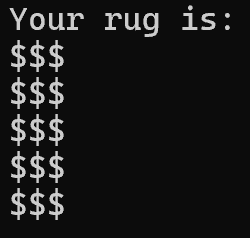
\includegraphics[height=1in]{./imgs/rug1_alt.PNG} \hspace{0.5in} \end{tabular}
			design\_run(16,5,\@) $\rightarrow$ \begin{tabular}{l}
			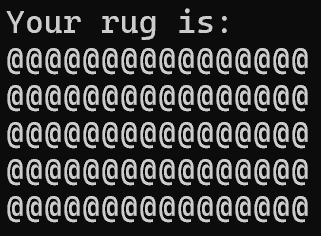
\includegraphics[height=1in]{./imgs/rug2_alt.PNG} \end{tabular}


%end_of_questions
%make sure to leave at least one blank line below

